\documentclass{article}

\title{Faculty Data Story}
\author{Henry Oehlrich}
\date{08-21-2023}

\usepackage[margin=1.25in]{geometry}
\usepackage{graphicx}
\usepackage{caption}
\usepackage{subcaption}
\graphicspath{{school/math/images/}}

\begin{document}

\maketitle{}

Thirty-four Raleigh Charter High School staff and faculty members responded to
a survey where they were asked to report on a variety of questions. One such
question was which color binder they associate most with History. The results
of which are shown in a pie chart and a bar chart in figure 1a and 1b
respectively. Both charts show that the color blue is the most popular color
associated with History. While both charts are based on the same data, the pie
chart shows far more clearly the percent of faculty that chose each color. The
bar chart, on the other hand, shows the raw number of faculty that chose each
color. The pie chart uses our eyes' abilities to associate both words and
colors with sizes rather than merely associate words with sizes as in the bar
chart.

\begin{figure}[h]
    \centering
    \begin{subfigure}{.5\textwidth}
        \centering
        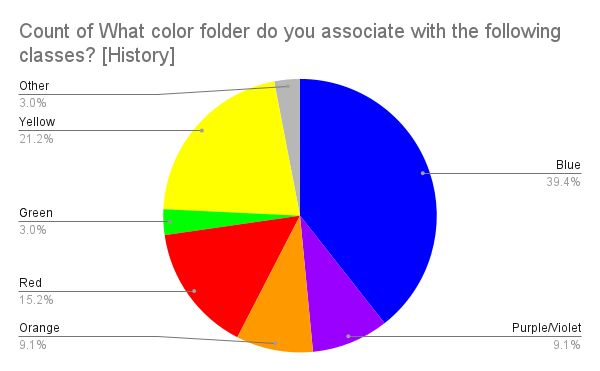
\includegraphics[width=\linewidth]{history-binder-color-pie.png}
        \caption{Pie chart}
        \label{fig:test1}
    \end{subfigure}%
    \begin{subfigure}{.5\textwidth}
        \centering
        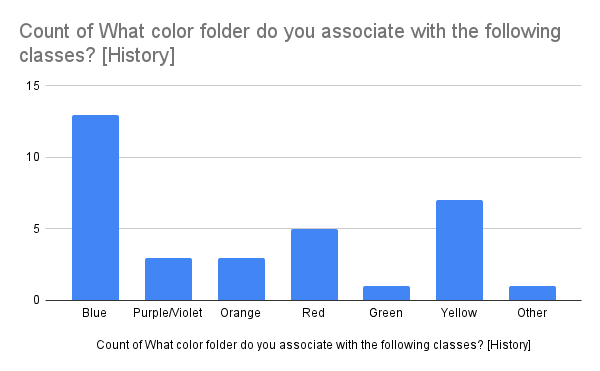
\includegraphics[width=\linewidth]{history-binder-color-bar.png}
        \caption{Bar chart}
        \label{fig:test2}
    \end{subfigure}
    \caption{Charts of the color folder RCHS faculty associated with History}
\end{figure}

\end{document}

